\documentclass[12pt,a4paper]{article}
\usepackage[pdftex]{graphicx}
\usepackage{url} 
\usepackage[bookmarks, colorlinks=false, pdfborder={0 0 0}, pdftitle={<pdf title here>}, pdfauthor={<author's name here>}, pdfsubject={<subject here>}, pdfkeywords={<keywords here>}]{hyperref} 
\usepackage{caption}
\usepackage{subcaption}
\usepackage{float}
\usepackage{multicol}
\usepackage[section]{placeins}
\usepackage{amsmath}
\usepackage{array}
\usepackage{multirow}
\usepackage{ragged2e}

% Paper margins etc.
\usepackage{geometry}
 \geometry{
 a4paper,
 total={170mm,257mm},
 left=20mm,
 top=20mm
 }

\begin{document}

\begin{titlepage}

\begin{center}

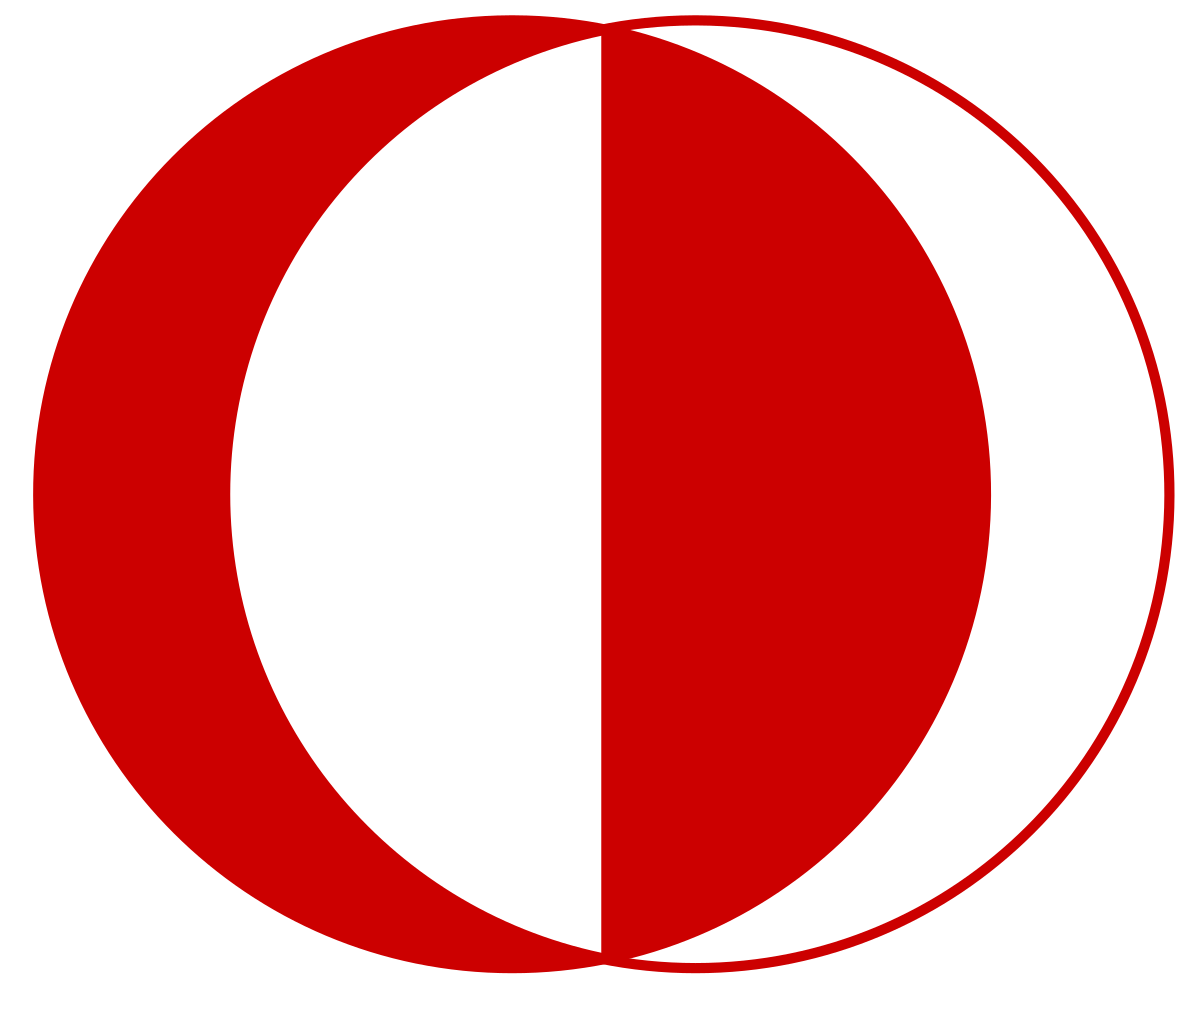
\includegraphics[width=0.3\textwidth]{Figures/metu_logo.png}\\
\vspace{.3in}
\textup{{\bf Middle East Technical University}}\\

% Title
\Large \textbf{EE464 Static Power Conversion II}\\[0.3in]
\Large \textbf{Hardware Project Simulation and Magnetic Design Report}\\

\noindent\rule{6cm}{0.4pt}

% Authors
\normalsize \textit{Submitted by Klerans:} \\

\vspace{.3in}

\textbf{İsa Ersöz}\\
\textbf{ID:} 2374908 \\
isa.ersoz@metu.edu.tr\\
%\textbf{tel:} 541 201 7310 \\

\vspace{.3in}

\textbf{Arda Kasım}\\
\textbf{ID:} 2232197\\
arda.kasim@metu.edu.tr\\
%\textbf{tel:} 541 201 7310 \\

\vspace{.3in}

\textbf{Fatih Erden}\\
\textbf{ID:} 2304566\\
fatih.erden@metu.edu.tr\\
%\textbf{tel:} 533 895 3807\\

\noindent\rule{6cm}{0.4pt}

\vspace{.3in}

\textbf{Submission Date:} \today

\end{center}

\end{titlepage}

\pagenumbering{arabic}

\tableofcontents

\listoffigures
\listoftables

\newpage
\section{Introduction}
In this project, it is aimed to build an isolated DC-DC converter. The specifications of the project is given in the below Table \ref{tab:project_specs} In this report, our thoughts on the potential topologies, their advantages and disadvantages are discussed. We have decided on building an isolated SEPIC converter whose circuit diagram can be seen in Figure \ref{fig:iso_sepic}. Then the team has decided on the transformer design and other components of the topology. Furthermore, computer simulations of the topology with ideal and non-ideal components are given.

% BURAYA TABLE ATICAZ
\begin{table}[H]
    \centering
    \caption{Project Specifications.}
    \label{tab:project_specs}
    \begin{tabular}{|c|c|}
        \hline
        Input Voltage               & 12-18 V   \\
        \hline
        Output Voltage              & 48 V      \\
        \hline
        Output Voltage Ripple       & 3\%       \\  
        \hline
        Output Power                & 48 W      \\
        \hline
        Line Regulation             & 3\%       \\
        \hline
        Load Regulation             & 3\%       \\
        \hline
    \end{tabular}
\end{table}

\section{Topology Selection}
Starting the design, the topology selection must be covered first. The five isolated DC-DC converter topologies that were covered in the lectures are listed with their strengths and weaknesses in Table \ref{tab:procon}\cite{web:keysan}.
\renewcommand{\arraystretch}{1.5}
\begin{table}[H]

\centering
\caption{Comparison of Isolated DC-DC Converter Topologies}
\label{tab:procon}
\begin{tabular}{|m{0.2\textwidth}<{\centering}|m{0.35\textwidth}|m{0.35\textwidth}|}
    \hline
    \textbf{Topology} & \centering \textbf{Advantages} & \centering \textbf{Disadvantages} \arraybackslash \\ \hline
    
    \multirow{4}{*}{Flyback} & $\bullet$ Two-winding transformer & $\bullet$ High MOSFET voltage stress\\
    & $\bullet$ Low component count & $\bullet$ Low controllability \\ 
    & $\bullet$ Analog ICs are available for the duty cycle control & $\bullet$ Needs snubber due to leakage and parasitic inductances at primary side \\ \hline
    
    \multirow{3}{*}{Forward} & \multirow{3}{0.35\textwidth}{\justifying $\bullet$ $L_m$ has a discharge path on the auxiliary winding, no need for transformer snubber} & $\bullet$ Utilizes a three-winding transformer, hard to implement by hand-winding \\
    & & $\bullet$ Has an additional inductor, may cause additional magnetic design work \\ \hline

    \multirow{4}{*}{Push-Pull} & $\bullet$ Core utilization of the transformer is better, core can be smaller in size & $\bullet$ Utilizes a centre-tap transformer, hard to implement by hand-winding \\
    & $\bullet$ Easier to filter at the output as the current and voltage waveforms ripple at twice the switching frequency & $\bullet$ Two switches to control with additional measures to consider such as dead-time \\  \hline

    Half-Bridge & \multirow{3}{0.35\textwidth}{\justifying $\bullet$ Similar considerations with Push-Pull such as better core utilization and easy filtering} & \multirow{3}{0.35\textwidth}{\justifying $\bullet$ Similar considerations with Push-Pull such as hard to implement transformer and multiple switches to control}  \\
    \& & & \\
    Full-Bridge &  &   \\  \hline
\end{tabular}
\end{table}
Considering the design challenges, the most difficult task will be the transformer implementation. It will be challenging to make transformer parameters match the simulated one, as it will be winded by hand. Therefore, choosing a topology with a simple two winding transformer would be more sensible. Moreover, flyback is the only option that is covered during the lectures utilizing a two winding transformer. \smallskip \\
Flyback could be our choice of topology, but we decided against it due to two reasons. Firstly, Flyback needs a snubber circuit which not only decreases efficiency but also an additional design process; which we are not so experienced with. Secondly, we want to work on a unique topology in order to get extra points. In order to find a topology suited to our needs, we made some more research. \smallskip \\
It is a common knowledge that Flyback converter was initially evolved from Buck-Boost converter by replacing the inductor with a transformer so that the isolation is achieved. We thought that there may be a similar derivation for SEPIC converter which also has an inductor with a connection to the return path just like the Buck-Boost Converter. We did our research to find out that there was indeed an isolated SEPIC converter which suits our previously mentioned needs which is shown in Figure \ref{fig:iso_sepic}.
\begin{figure}[h]
    \centering
    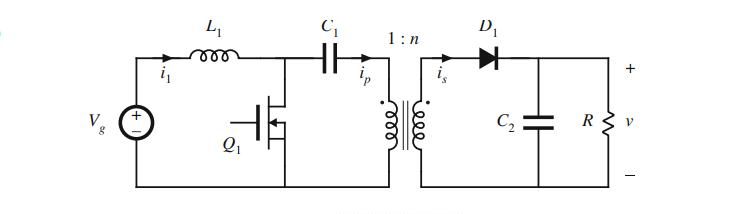
\includegraphics[width=\textwidth]{Figures/isolated_sepic.png}
    \caption{Isolated SEPIC Converter}
    \label{fig:iso_sepic}
\end{figure} \\
Some design considerations regarding isolated SEPIC converter can be stated as
\begin{itemize}
    \item The transformer acts similarly to the Flyback transformer, which sends power during off cycle.
    \item $C_1$ must be very large (ideally infinite).
    \item Assuming the previous requirement is met, $V_{C_1}$ $\approx$ $V_g$ and almost constant.
    \item Assuming $V_{C_1}$ = $V_g$, $I_{L_1}$ and $I_{L_m}$ have exactly the same voltage waveforms  during both the switch on and off cycles. If the magnetic design is done such that $L_1$ $\approx$ $L_m$, their current waveforms will almost be identical too. Therefore, measuring and controlling the current (if desired) from the input will be enough to control transformer current as well.
    \item $I_{Q_1}$ is approximately twice the input current during the on cycle, assuming $L_1$ $\approx$ $L_m$.
    \item Assuming ideal components, MOSFET blocking voltage can be found as $V_{Q_1}$ = $V_g$ + $V_o/n$. Overshoots during the switching instants must be considered as well.
\end{itemize}
The voltage transfer ratio for an isolated SEPIC converter can be stated as
\begin{equation*}
    \frac{V_o}{V_s} = \frac{N_2}{N_1}\frac{D}{1-D}
\end{equation*}
After evaluating positives and negatives we have decided to go for an isolated SEPIC converter design for the project.

\section{Magnetic Design}

\subsection{Wire Selection}
To select the proper wires for transformer windings and inductor coil, we considered the average ratings of input and output currents. Also the skin effect ()is taken into account. Therefore looking at the AWG table (BURAYA REF) , we have selected the 26AWG. Parameters of the cable are given in Table \ref{tab:AWG26} 

\begin{table}[H]
    \centering
    \caption{AWG26 cupper conductor parameters.(REF)}
    \label{tab:AWG26}
    \begin{tabular}{|c|c|}
        \hline
        Max. Amp rate:                          & 0.361 $A$   \\
        \hline
        Conductor diameter:                     & 0.4 $mm$    \\
        \hline
        Conductor cross-section area:           & 0.128 $mm^2$\\
        \hline
        Max. frequency for 100\% skin depth:    & 107 $kHz$   \\
        \hline
    \end{tabular}   
\end{table}

Since its Amp. rate is very low but it gives 100\% skin depth, we can parallel this wire for our primary and secondary windings. Considering the worst case scenario of 12 V input (giving 4 A input current), and accounting for the 10\% losses on the design, we can assume that input current will be around 4.4 A. For the output side it is assumed to be around 1 A output current for 48 W output power.

\begin{table}[H]
    \centering
    \caption{Transformer Wiring Configuration.}
    \label{tab:tr_wiring}
    \begin{tabular}{|c|c|c|}
        \hline
        Transformer side            & Assumed Current level & \# of parallel wires   \\
        \hline\hline
        Primary                     & 4.4 A                 & 12                    \\
        \hline
        Secondary                   & 1 A                   & 3                     \\
        \hline
    \end{tabular}
\end{table}


\subsection{Core Selection}
We first decided on core geometry considering the recommendations from Ferrite Core Catalog by the Magnetics \cite{web:ferrite_cores}. As the winding of the transformer is a topic that we are not very familiar of, we filtered our geometries to the ones that have a cylindrical winding surface to simplify the process. ETD core shape seemed to be best fit for our application and it is recommended for transformers by the catalog. \\
After doing some market research, we quickly realized that only ferrite cores are available to purchase in Turkey. Therefore, we decided to base our design for a ferrite core; so that we can quickly purchase a new core in case of an emergency. Ferrite cores also have a linear B-H characteristics until they are saturated, which simplifies the design process. \\
Considering the area that the windings occupy we have chosen ETD39 sized core to stay below a fill factor of 0.3.
\subsection{Transformer Design}
As the voltage transfer ratio has a $\frac{D}{1-D}$ dependence, we needed to fix our duty cycle range around 0.5 for a safe operation. Therefore, we decided on a duty cycle range of 0.4 $<$ D $<$ 0.6. We also chose $f_{sw}=50$kHz as we not only believe it is a sweet-spot for the choice of switching frequency but also provides some margin for an increase in frequency until skin effect is observed at the wires. This margin may become useful during the implementation as real-world effects may lead us to increase the switching frequency.  \\
We can calculate the required turns ratio for the extremities of the duty cycle and the input voltage as
\begin{equation*} \medskip \\
    \frac{48}{12} = \frac{N_2}{N_1} \frac{0.6}{1-0.6}
\end{equation*}
\begin{equation*} \medskip \\
    \frac{N_2}{N_1} = 2.67
\end{equation*}
\begin{equation*} \medskip \\
    \frac{48}{18} = \frac{N_2}{N_1} \frac{0.4}{1-0.4}
\end{equation*}
\begin{equation*} \medskip \\
    \frac{N_2}{N_1} = 1.78
\end{equation*}
As there will be some losses as well, choosing a turns ratio a little over the larger result would ensure the operation stays at 0.4 $<$ D $<$ 0.6. We chose our turns ratio to be 3.2 (i.e. 5:16), around 1.2 times the calculated turns ratio. Furthermore, we also assumed $\Delta i_{L_m} = 2i_{L_m,avg} = 8$A, to find the minimum inductance required for CCM operation. \\
We can write the inductor charging and discharging equations for 12V input (worst case), assuming ideal components and without explicitly stating duty cycles as
\begin{equation*}
    V_s D T_s = L_m \Delta i_{L_m}
\end{equation*}
\begin{equation*}
    D = \frac{L_m \Delta i_{L_m} f_{sw}}{V_s}
\end{equation*}
\begin{equation*}
    D = \frac{L_m \times 8 \times 50k}{12}
\end{equation*}
\begin{equation} \bigskip \\
    D = 33333.33 \; L_m
\end{equation}
\begin{equation*}
    \frac{V_o (1-D) T_s N_1}{N_2} = L_m \Delta i_{L_m}
\end{equation*}
\begin{equation*}
    1-D = \frac{L_m \Delta i_{L_m} f_{sw} N_2}{V_o N_1}
\end{equation*}
\begin{equation*}
    1-D = \frac{L_m \times 8 \times 50k \times 3.2}{48}
\end{equation*}
\begin{equation} \medskip \\
    1-D = 26666.67 \; L_m
\end{equation}
Adding equations (1) and (2) we get
\begin{equation*} \medskip \\
    1 = 60000 \; L_m
\end{equation*}
\begin{equation*} \medskip \\
    L_m = 16.67 \; \mu H
\end{equation*}
for CCM-DCM border operation. \\
We multiplied this number by 1.5 so that we are guaranteed to operate at CCM. Thus, $L_m = 25 \; \mu H$ can be stated as the absolute minimum inductance required. At this stage the core choice must be finalized in order to continue the design. \\
To select a suitable core we must either fix the operating flux density and find the primary number of turns or fix the number of turns and make sure that core does not saturate. We chose the second option and fixed the number of turns for the transformer as
\begin{equation*}
    N_p = 10, \; N_s = 32
\end{equation*}
Then we can calculate the total area the wires will occupy as
\begin{equation*}
    A_{wire} =  0.128 mm^2 \times [(12\times10)+(32\times3)] = 27.65 mm^2
\end{equation*}
Taking fill factor into account, we determined that both ETD34 and ETD39 sized cores are suitable for hand-winding. Core suppliers produce fixed various gapped versions of the cores as well as their inductance factors and effective permeabilities given in the datasheet for each version. The purpose behind this methodology was to avoid using a custom determined gap, which would be time consuming to implement accurately.\\
We quickly calculated the operating points for several different gap values and came up with a possible configuration for each size. \medskip \\
$\bullet$ ETD34 Core, g = 0.2mm, $A_L$ = 482 $nH/T^2$, $\mu_e$ = 310, $l_e$ = 78.6mm
\begin{equation*}
    L_m = A_L \times N_p^2 = 482n \times 100 = 48.2 \mu H
\end{equation*}
Similar derivation with equations (1) and (2)
\begin{equation*}
    D = \frac{L_m \Delta i_{L_m} f_{sw}}{V_s}
\end{equation*}
\begin{equation*}
    D = \frac{48.2\mu \times \Delta i_{L_m} \times 50k}{12}
\end{equation*}
\begin{equation}
    D = 0.2 \; \Delta i_{L_m}
\end{equation}
\begin{equation*}
    1-D = \frac{L_m \Delta i_{L_m} f_{sw} N_2}{V_o N_1}
\end{equation*}
\begin{equation*}
    1-D = \frac{48.2\mu \times \Delta i_{L_m} \times 50k \times 3.2}{48}
\end{equation*}
\begin{equation}  \\
    1-D = 0.16 \; \Delta i_{L_m}
\end{equation}
Adding equations (3) and (4) we get
\begin{equation*}  \\
    1 = 0.36 \; \Delta i_{L_m}
\end{equation*}
\begin{equation*}  \\
    \Delta i_{L_m} = 2.78 \; A
\end{equation*}
Then the maximum current can be found as
\begin{equation*}
    i_{L_m,max} = i_{L_m,avg} \times 1.1 + \Delta i_{L_m}/2 = 4 \times 1.1 + 1.4 = 5.8 \; A
\end{equation*}
where 1.1 multiplier is used as a safety margin. Using this result and applying Ampere's Law we can find the operating magnetic field of the core as
\begin{equation*}
    H \times l_e = N_p \times i_{L_m,max}
\end{equation*}
\begin{equation*}
    H = \frac{10 \times 5.8}{78.6 \times 10^{-3}} = 700 \; A/m
\end{equation*}
The magnetic flux density for this operating point can be found as
\begin{equation*}
    B = \mu_e H = 310 \times 4\pi \times 10^{-7} \times 700 = 0.272 \; T
\end{equation*}

$\bullet$ ETD39 Core, g = 0.5mm, $A_L$ = 326 $nH/T^2$, $\mu_e$ = 191, $l_e$ = 92.2mm
\begin{equation*}
    L_m = A_L \times N_p^2 = 326n \times 100 = 32.6 \mu H
\end{equation*}
Similar derivation with equations (1) and (2)
\begin{equation*}
    D = \frac{L_m \Delta i_{L_m} f_{sw}}{V_s}
\end{equation*}
\begin{equation*}
    D = \frac{32.6\mu \times \Delta i_{L_m} \times 50k}{12}
\end{equation*}
\begin{equation}
    D = 0.136 \; \Delta i_{L_m}
\end{equation}
\begin{equation*}
    1-D = \frac{L_m \Delta i_{L_m} f_{sw} N_2}{V_o N_1}
\end{equation*}
\begin{equation*}
    1-D = \frac{32.6\mu \times \Delta i_{L_m} \times 50k \times 3.2}{48}
\end{equation*}
\begin{equation}  \\
    1-D = 0.109 \; \Delta i_{L_m}
\end{equation}
Adding equations (5) and (6) we get
\begin{equation*}  \\
    1 = 0.245 \; \Delta i_{L_m}
\end{equation*}
\begin{equation*}  \\
    \Delta i_{L_m} = 4.08 \; A
\end{equation*}
Then the maximum current can be found as
\begin{equation*}
    i_{L_m,max} = i_{L_m,avg} \times 1.1 + \Delta i_{L_m}/2 = 4 \times 1.1 + 2.1 = 6.5 \; A
\end{equation*}
where 1.1 multiplier is used as a safety margin. Using this result and applying Ampere's Law we can find the operating magnetic field of the core as
\begin{equation*}
    H \times l_e = N_p \times i_{L_m,max}
\end{equation*}
\begin{equation*}
    H = \frac{10 \times 6.5}{92.2 \times 10^{-3}} = 705 \; A/m
\end{equation*}
The magnetic flux density for this operating point can be found as
\begin{equation*}
    B = \mu_e H = 191 \times 4\pi \times 10^{-7} \times 705 = 0.17 \; T
\end{equation*}
Both of the options suit the operation; however, ETD34 core option is very close to its saturation point. Hence, it can be risky to use that design for our project. We will use for the bigger core with the consequence of having high magnetic losses. \smallskip \\
Calculating the fill factor for the selected ETD39 core we get 
\begin{equation*}
    FF = \frac{A_{wire}}{A_e} = \frac{27.65 \; mm^2}{125 \; mm^2} = 0.22
\end{equation*}
Minimum transformer average current before the converter starts operating in DCM can be stated as
\begin{equation*}
    i_{L_m,avg,min} = \Delta i_{L_m}/2 = 2.04 \; A 
\end{equation*}
Therefore the minimum average load current can be found reflecting this value to the secondary side with the turns ratio as
\begin{equation*}
    i_{o,avg,min} = i_{L_m,avg,min}/3.2 = 2.04/3.2 = 0.6375 \; A 
\end{equation*}
The minimum transformer current at the CCM-DCM border is 0V as expected, whereas the maximum transformer current is equal to ripple current; which is 4.08A (ignoring current direction).

\section{Computer Simulations}  \label{comp_simulation}
\begin{figure}[H]
    \centering
    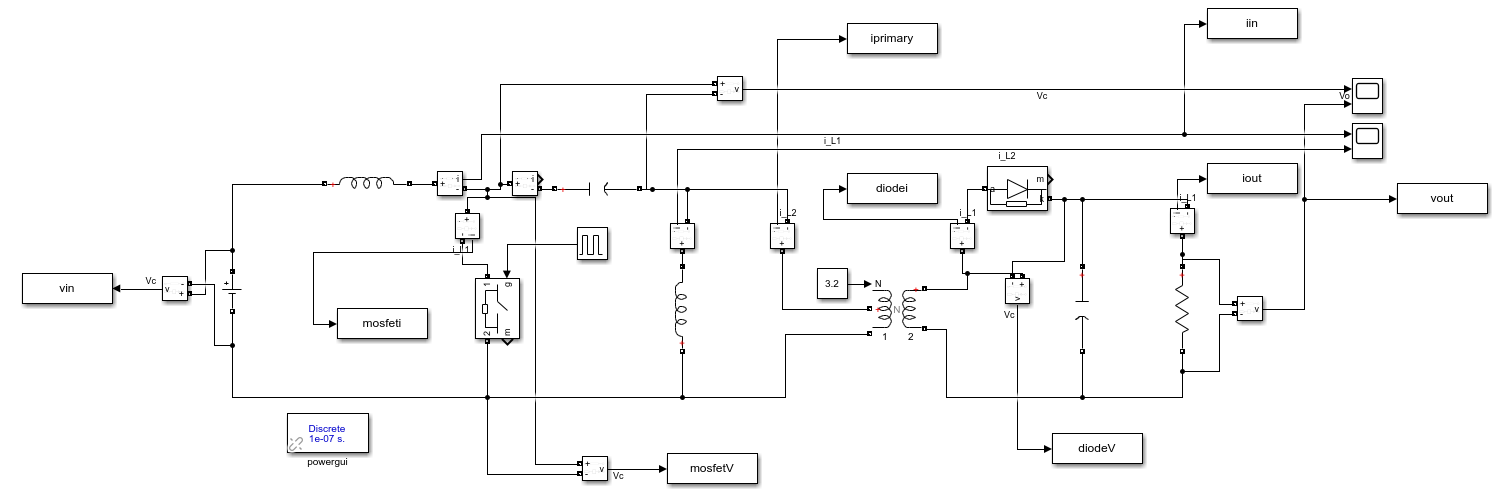
\includegraphics[width=\textwidth]{Figures/mat_cirr.png}
    \caption{Simulink simulation circuit for ideal case.}
    \label{fig:simulink}
\end{figure}
\begin{figure}[H]
    \centering
    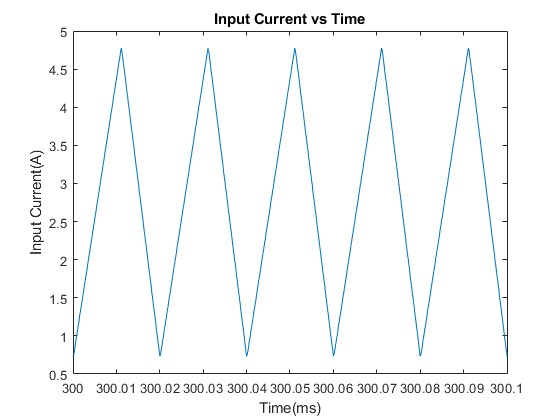
\includegraphics[width=0.6\textwidth]{Figures/mat_iin.jpg}
    \caption{$I_{in}$ versus time graph ideal case.}
    \label{fig:mat_i_in}
\end{figure}
\begin{figure}[H]
    \centering
    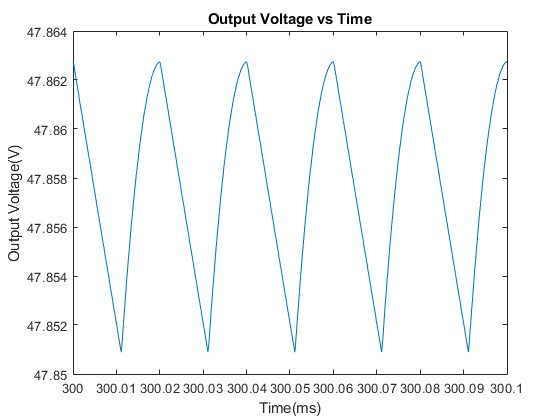
\includegraphics[width=0.6\textwidth]{Figures/mat_vout.jpg}
    \caption{$V_{out}$ versus time graph ideal case.}
    \label{fig:mat_v_out}
\end{figure}
\begin{figure}[H]
    \centering
    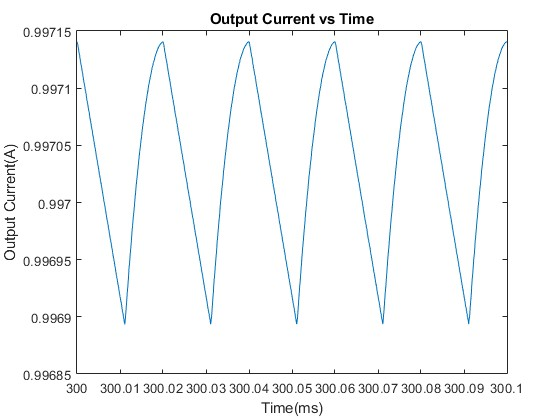
\includegraphics[width=0.6\textwidth]{Figures/mat_iout.jpg}
    \caption{$I_{out}$ versus time graph ideal case.}
    \label{fig:mat_i_out}
\end{figure}
\begin{figure}[H]
    \centering
    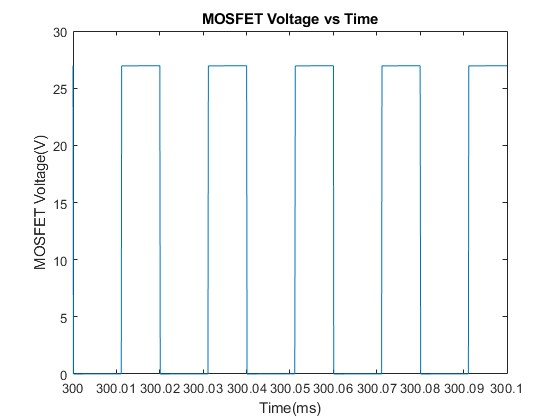
\includegraphics[width=0.6\textwidth]{Figures/mat_mos_volt.jpg}
    \caption{MOSFET voltage versus time graph ideal case.}
    \label{fig:mat_v_sw}
\end{figure}
\begin{figure}[H]
    \centering
    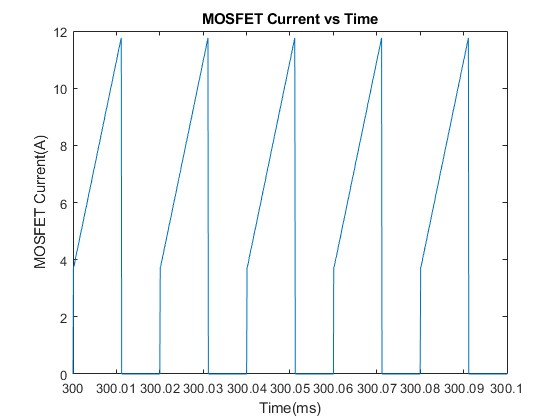
\includegraphics[width=0.6\textwidth]{Figures/mat_mos_curr.jpg}
    \caption{MOSFET current versus time graph ideal case.}
    \label{fig:mat_i_sw}
\end{figure}
\begin{figure}[H]
    \centering
    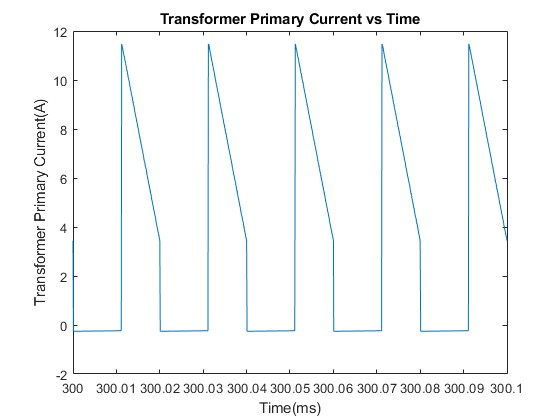
\includegraphics[width=0.6\textwidth]{Figures/mat_prim_current.jpg}
    \caption{Current on the transformer primary winding versus time ideal case.}
    \label{fig:mat_lm}
\end{figure}
\begin{figure}[H]
    \centering
    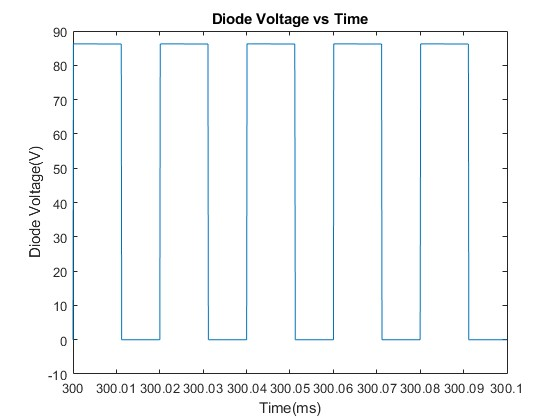
\includegraphics[width=0.6\textwidth]{Figures/mat_diode_volt.jpg}
    \caption{Diode voltage versus time graph ideal case.}
    \label{fig:mat_v_d}
\end{figure}
\begin{figure}[H]
    \centering
    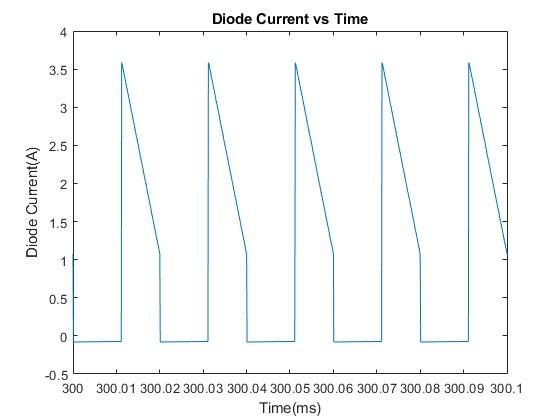
\includegraphics[width=0.6\textwidth]{Figures/mat_diode_current.jpg}
    \caption{Diode current versus time graph ideal case.}
    \label{fig:mat_i_d}
\end{figure}
\begin{figure}[H]
    \centering
    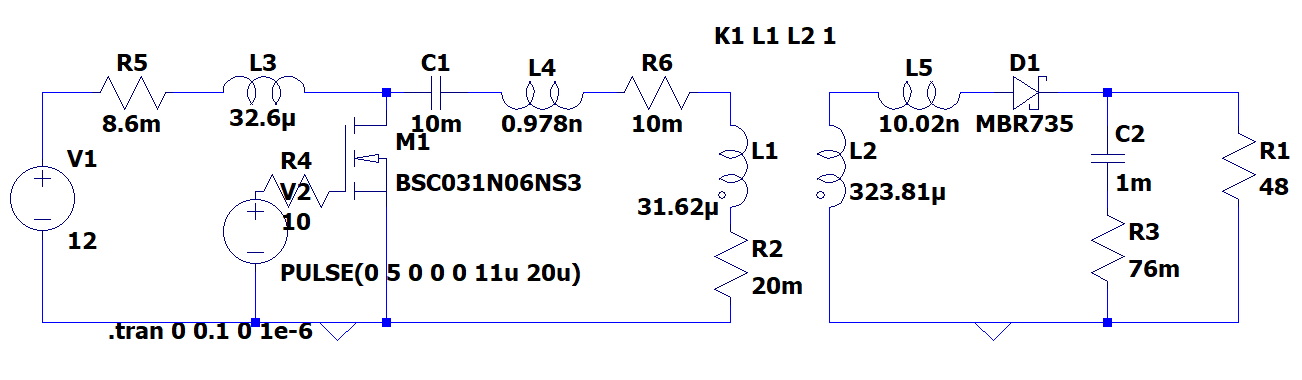
\includegraphics[width=\textwidth]{Figures/spice_circuit.png}
    \caption{LTSpice Circuit Diagram used for simulating the circuit with parasitic.}
    \label{fig:spice}
\end{figure}
\begin{figure}[H]
    \centering
    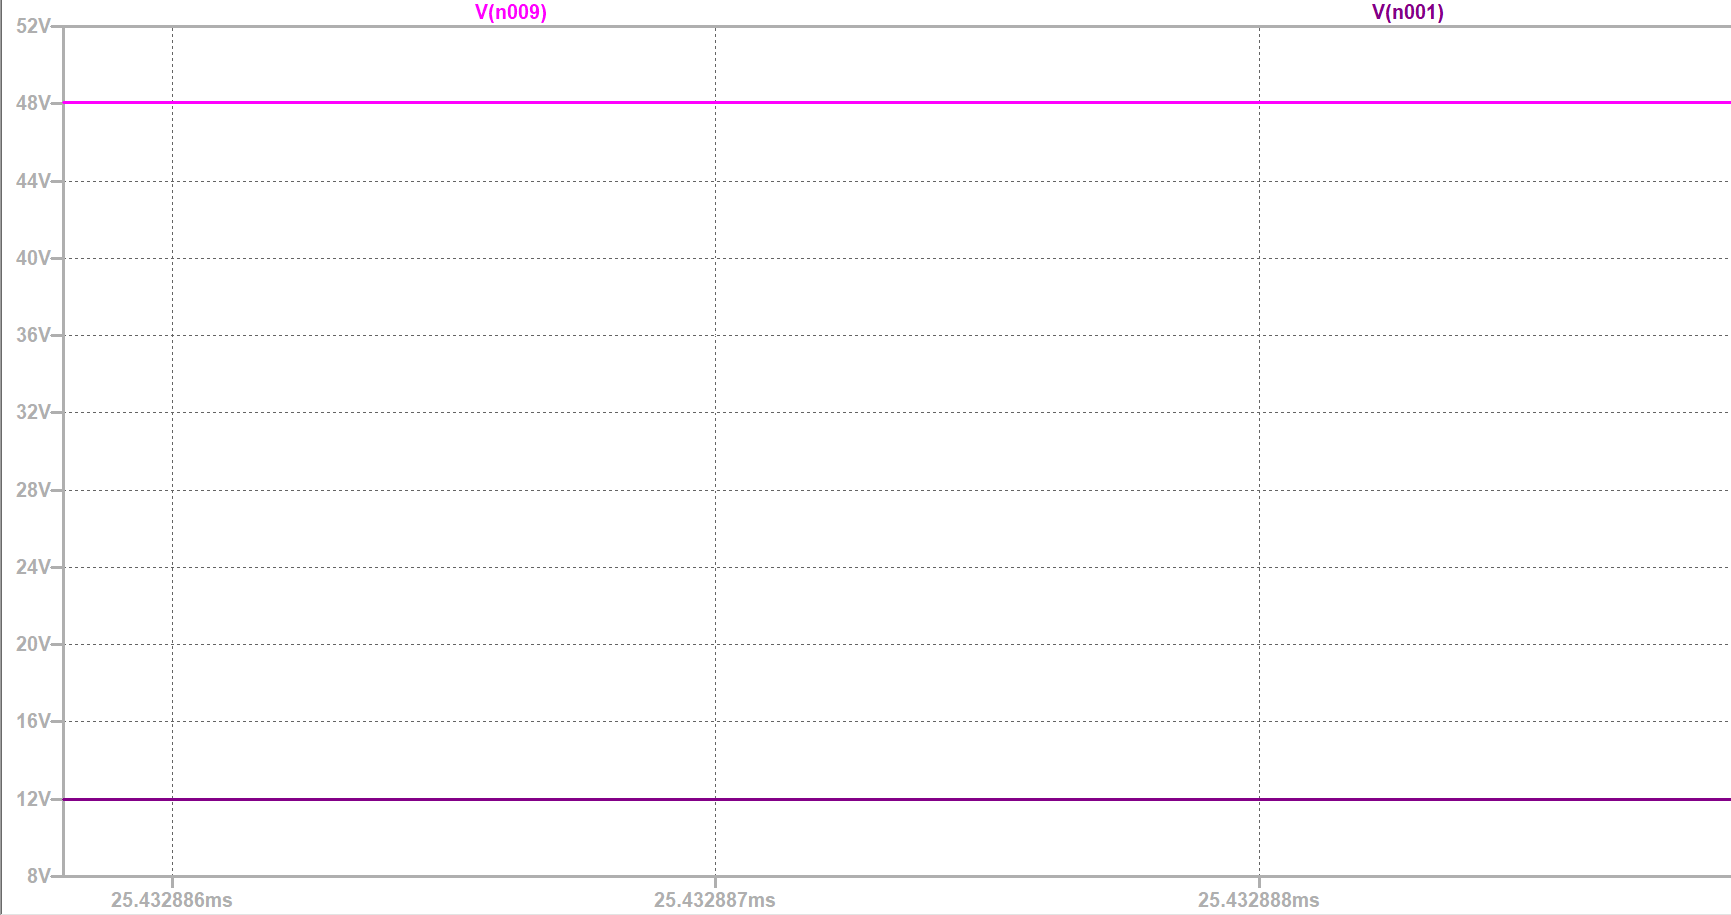
\includegraphics[width=0.6\textwidth]{Figures/vout-vin.png}
    \caption{$V_{out}$ and $V_{in}$ with parasitic included.}
    \label{fig:v_out_v_in}
\end{figure}
\begin{figure}[H]
    \centering
    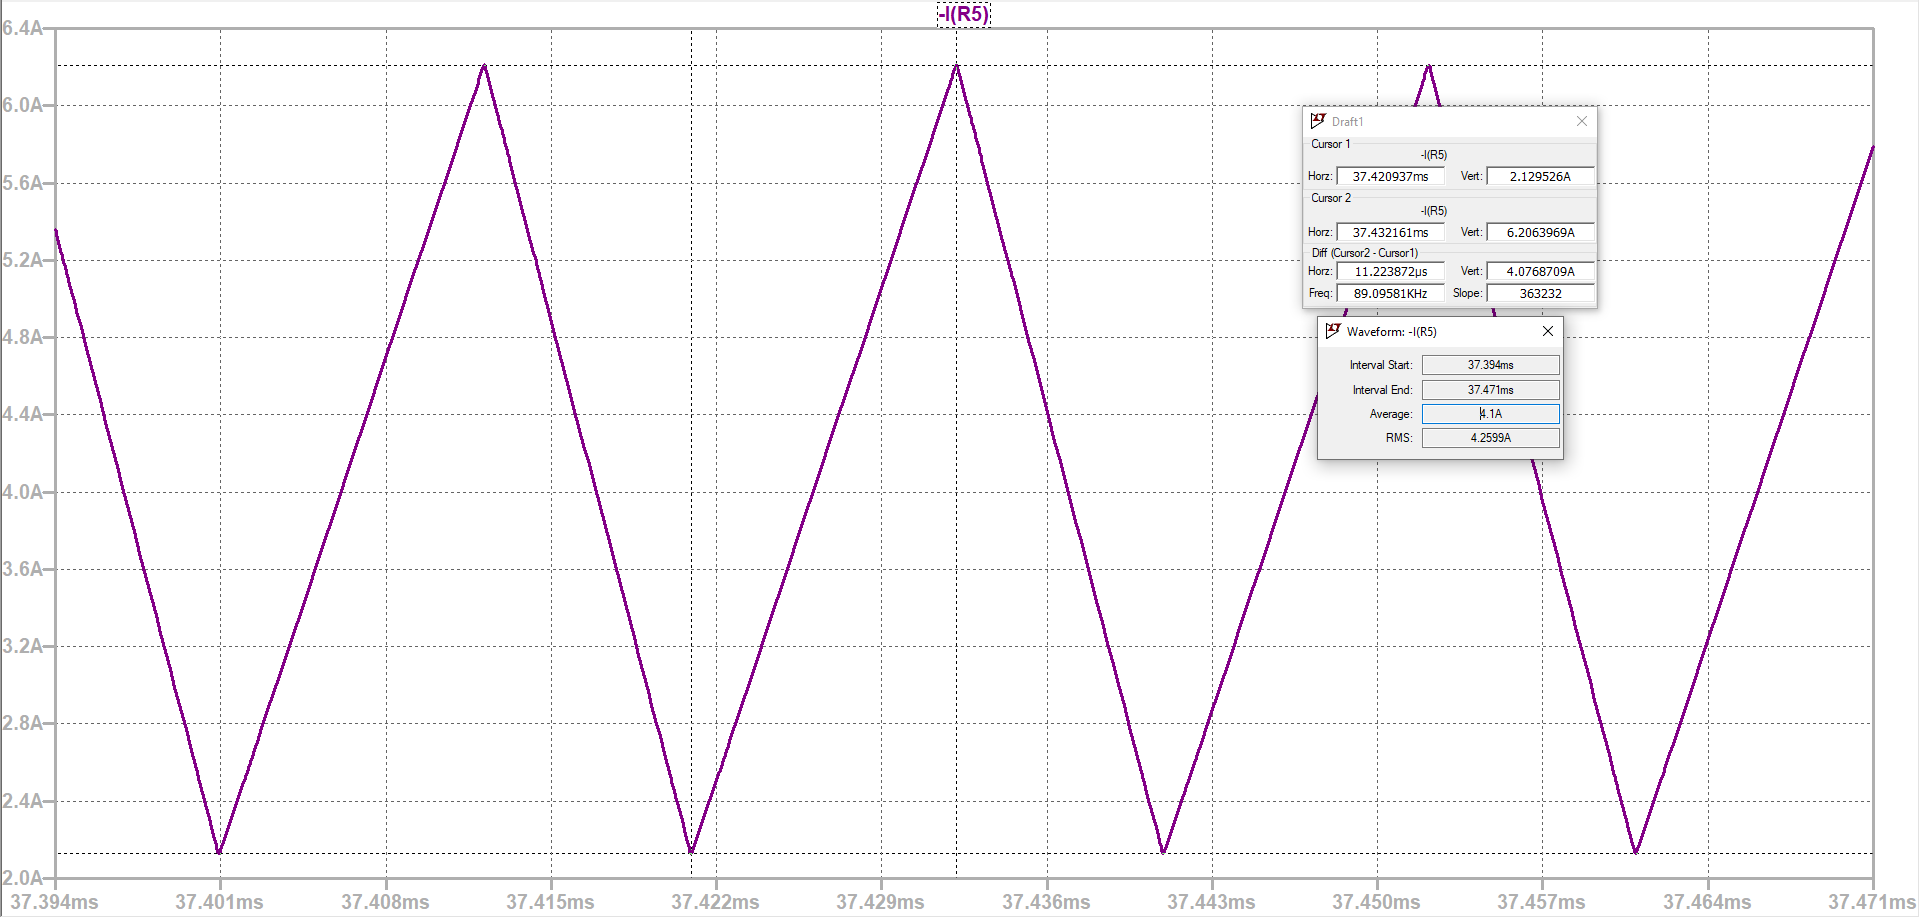
\includegraphics[width=0.6\textwidth]{Figures/in-av-ripple.png}
    \caption{$I_{in}$ waveform with parasitic included.}
    \label{fig:i_in}
\end{figure}
\begin{figure}[H]
    \centering
    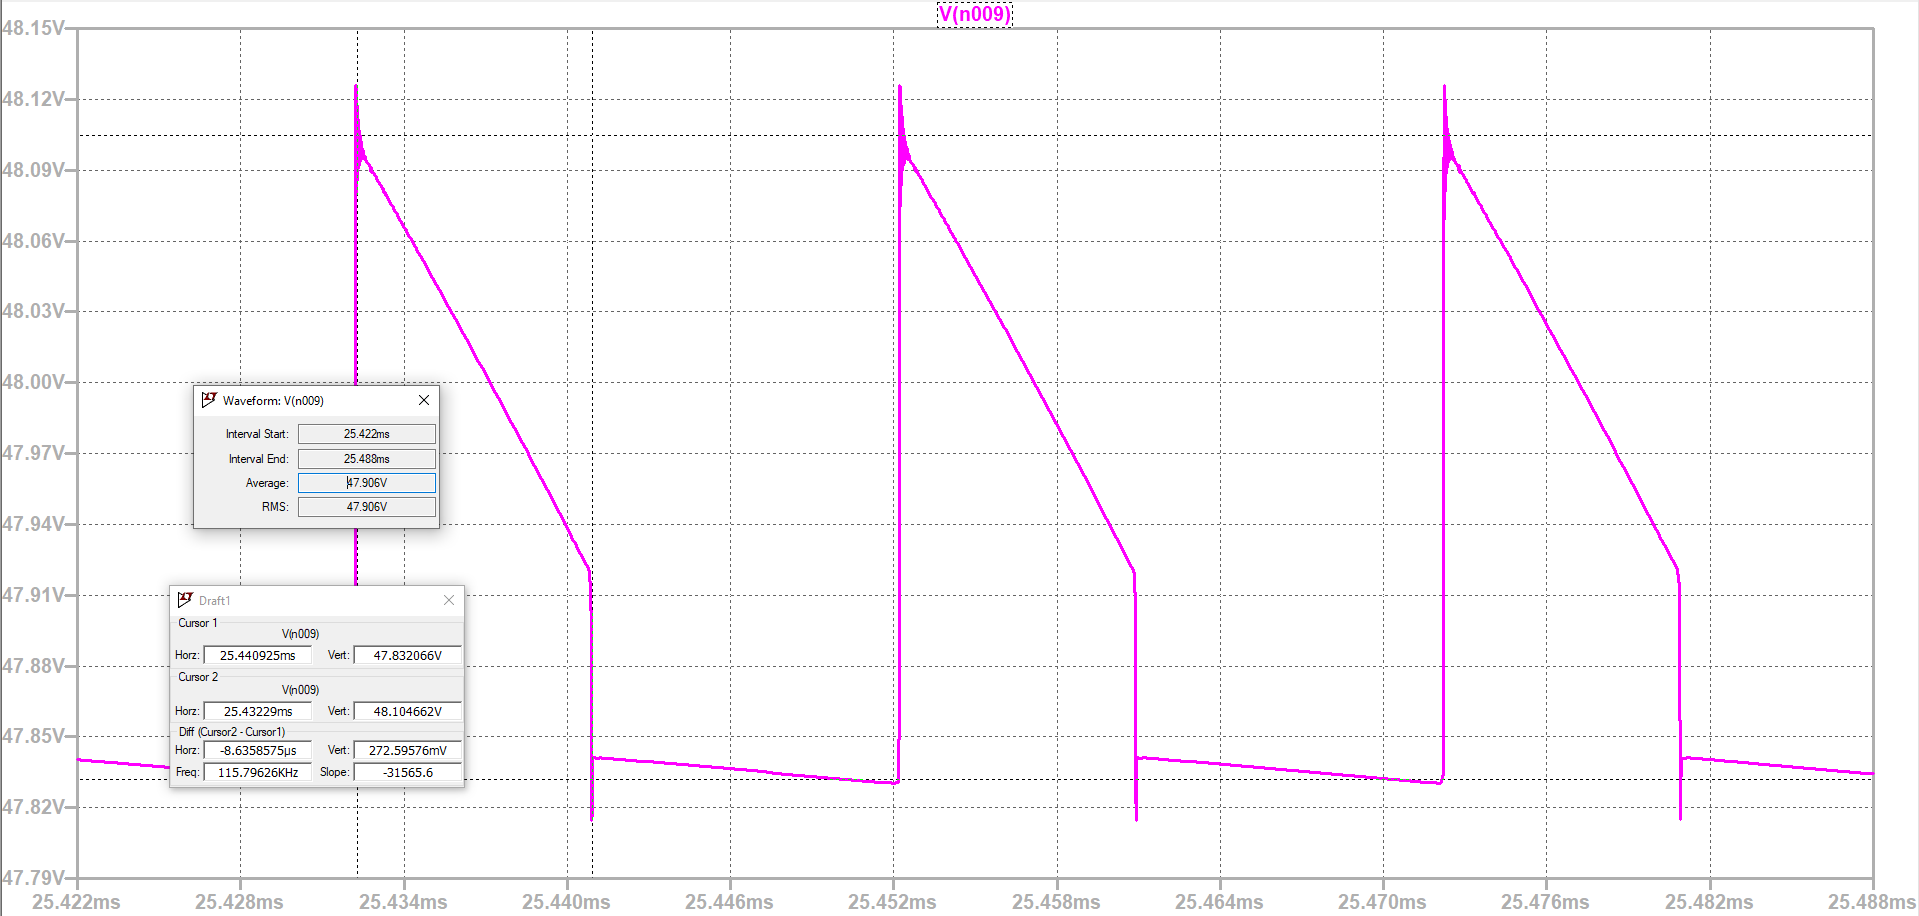
\includegraphics[width=0.6\textwidth]{Figures/vout-av-ripple.png}
    \caption{$V_{out}$ waveform with parasitic included.}
    \label{fig:v_out}
\end{figure}
\begin{figure}[H]
    \centering
    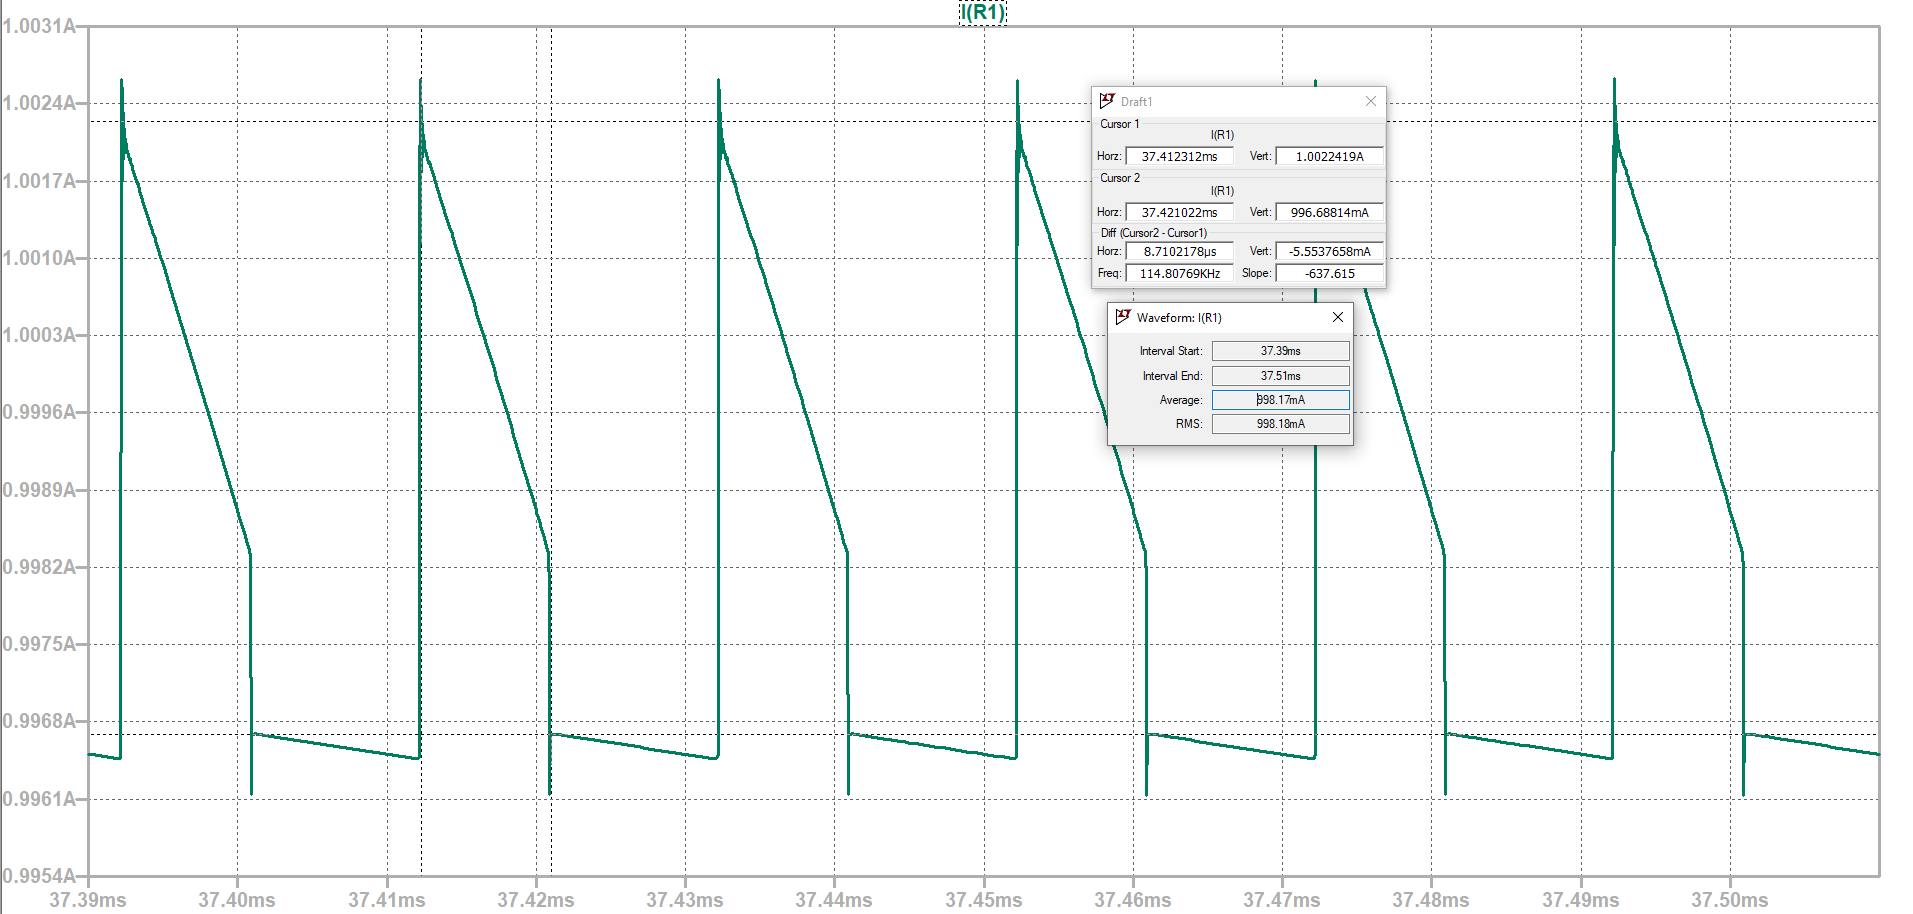
\includegraphics[width=0.6\textwidth]{Figures/iot-avg-ripple.png}
    \caption{$I_{out}$ waveform with parasitic included.}
    \label{fig:i_out}
\end{figure}
\begin{figure}[H]
    \centering
    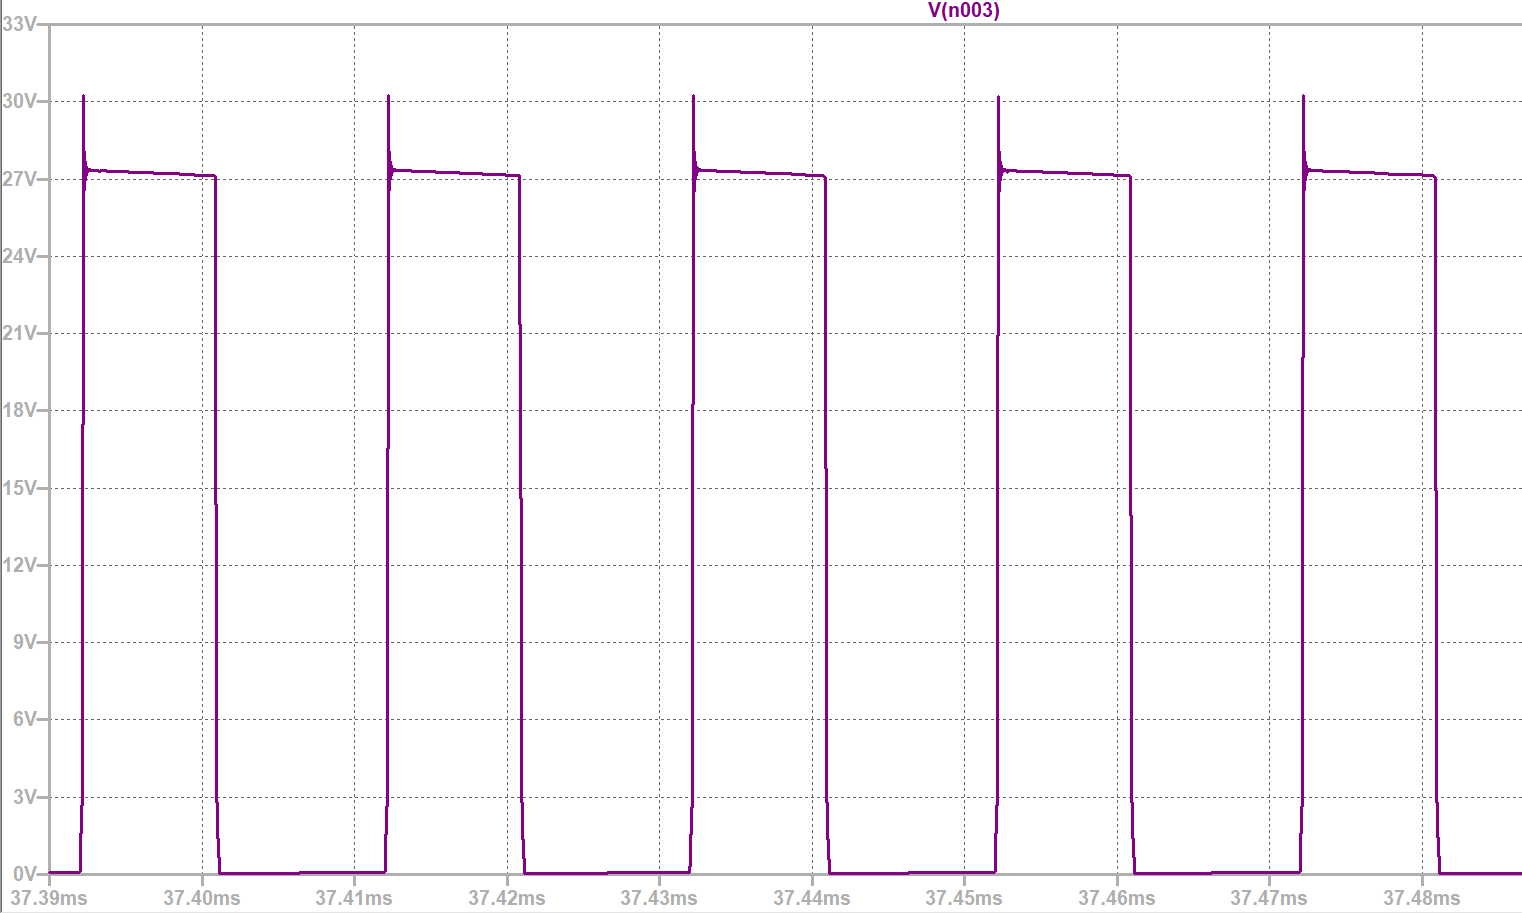
\includegraphics[width=0.6\textwidth]{Figures/mosfet-voltage.png}
    \caption{$V_{Q_1}$ waveform with parasitic included.}
    \label{fig:v_sw}
\end{figure}
\begin{figure}[H]
    \centering
    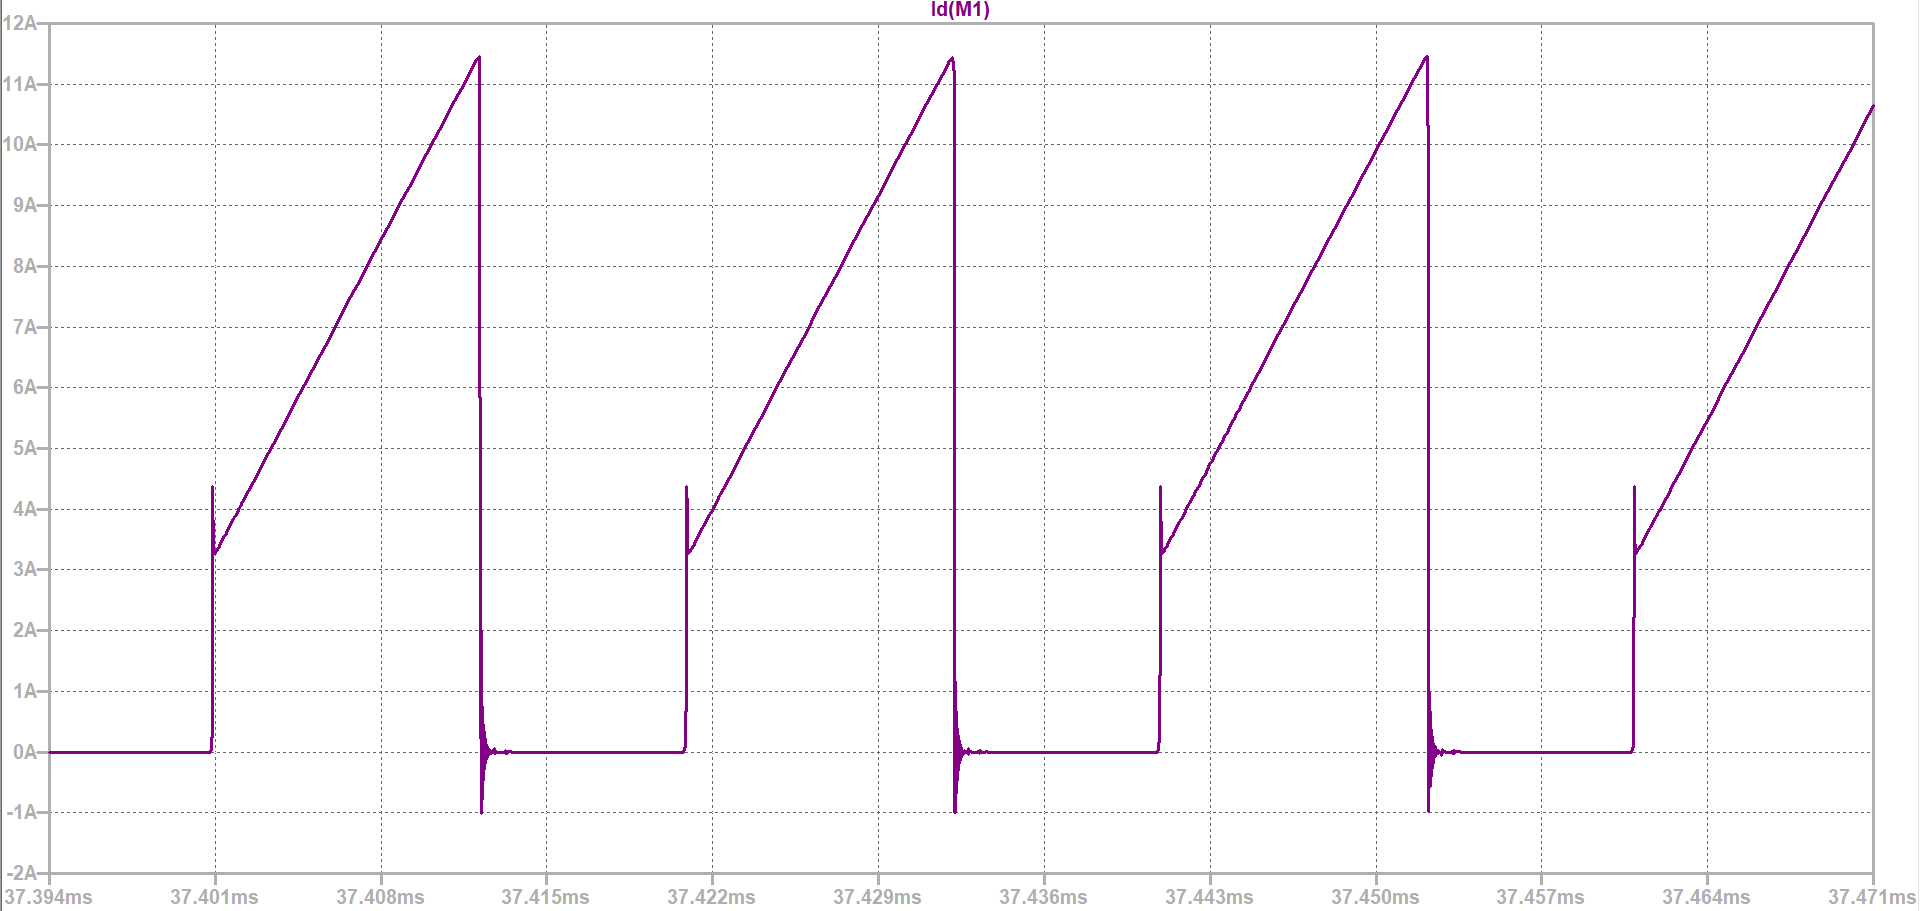
\includegraphics[width=0.6\textwidth]{Figures/mosfet-current.png}
    \caption{$I_{Q_1}$ waveform with parasitic included.}
    \label{fig:i_sw}
\end{figure}
\begin{figure}[H]
    \centering
    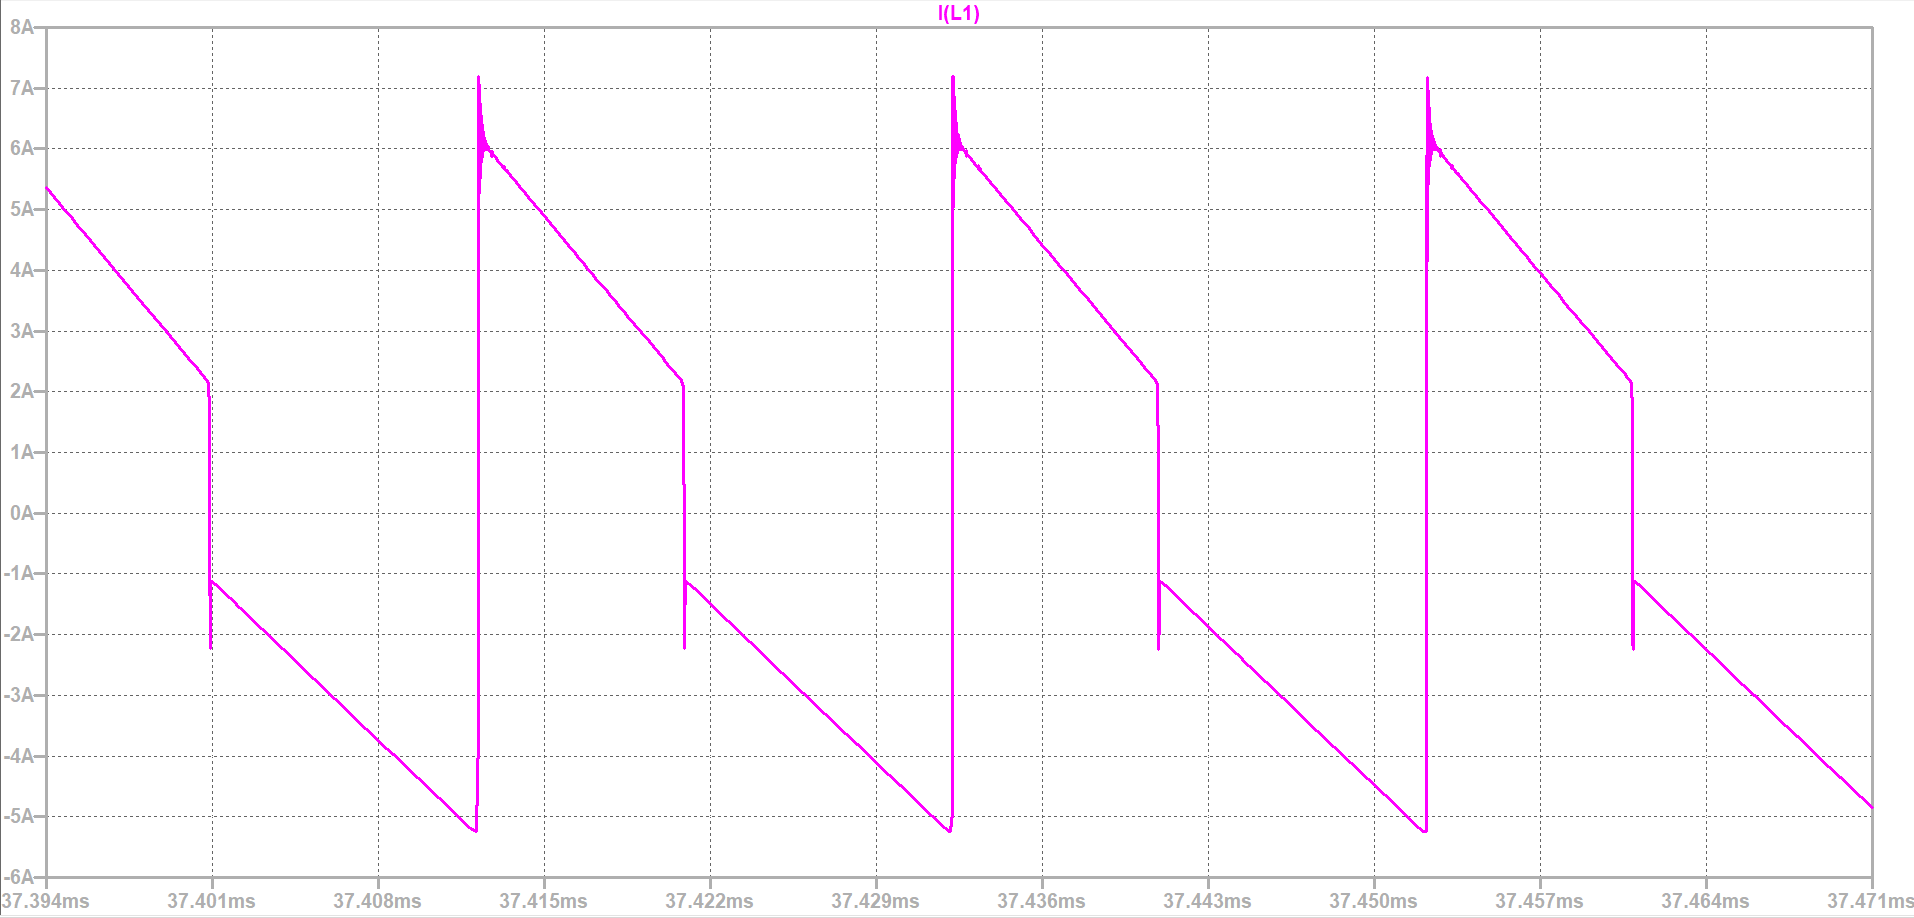
\includegraphics[width=0.6\textwidth]{Figures/trans_prim_curr.png}
    \caption{Caption}
    \label{fig:lm}
\end{figure}
\begin{figure}[H]
    \centering
    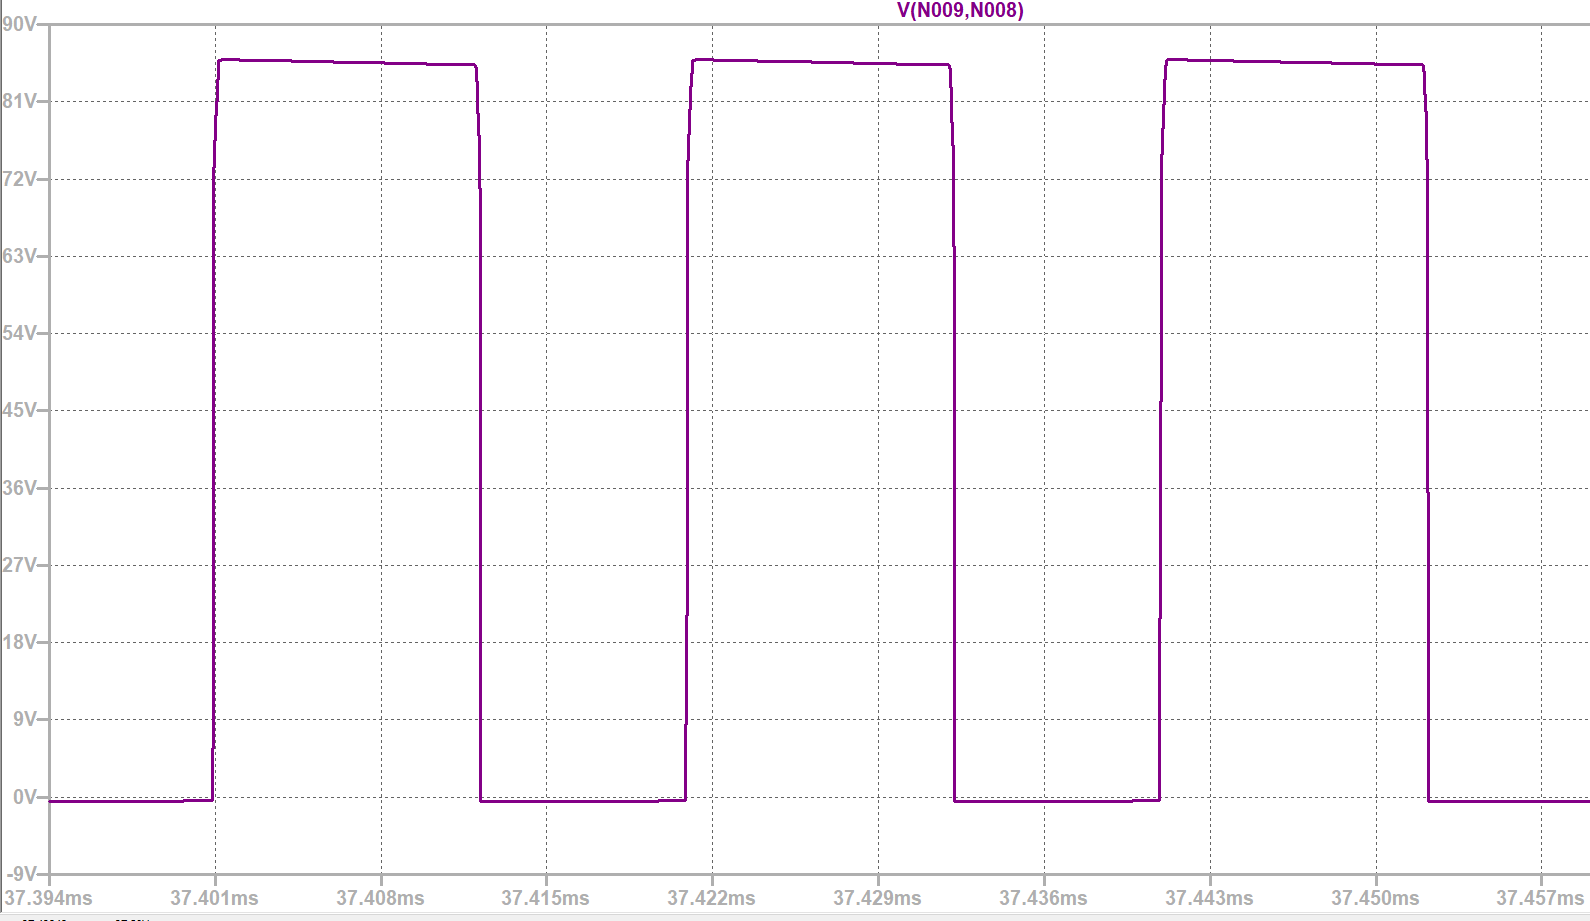
\includegraphics[width=0.6\textwidth]{Figures/diode-voltage.png}
    \caption{$V_{D_1}$ waveform with parasitic included.}
    \label{fig:v_d}
\end{figure}
\begin{figure}[H]
    \centering
    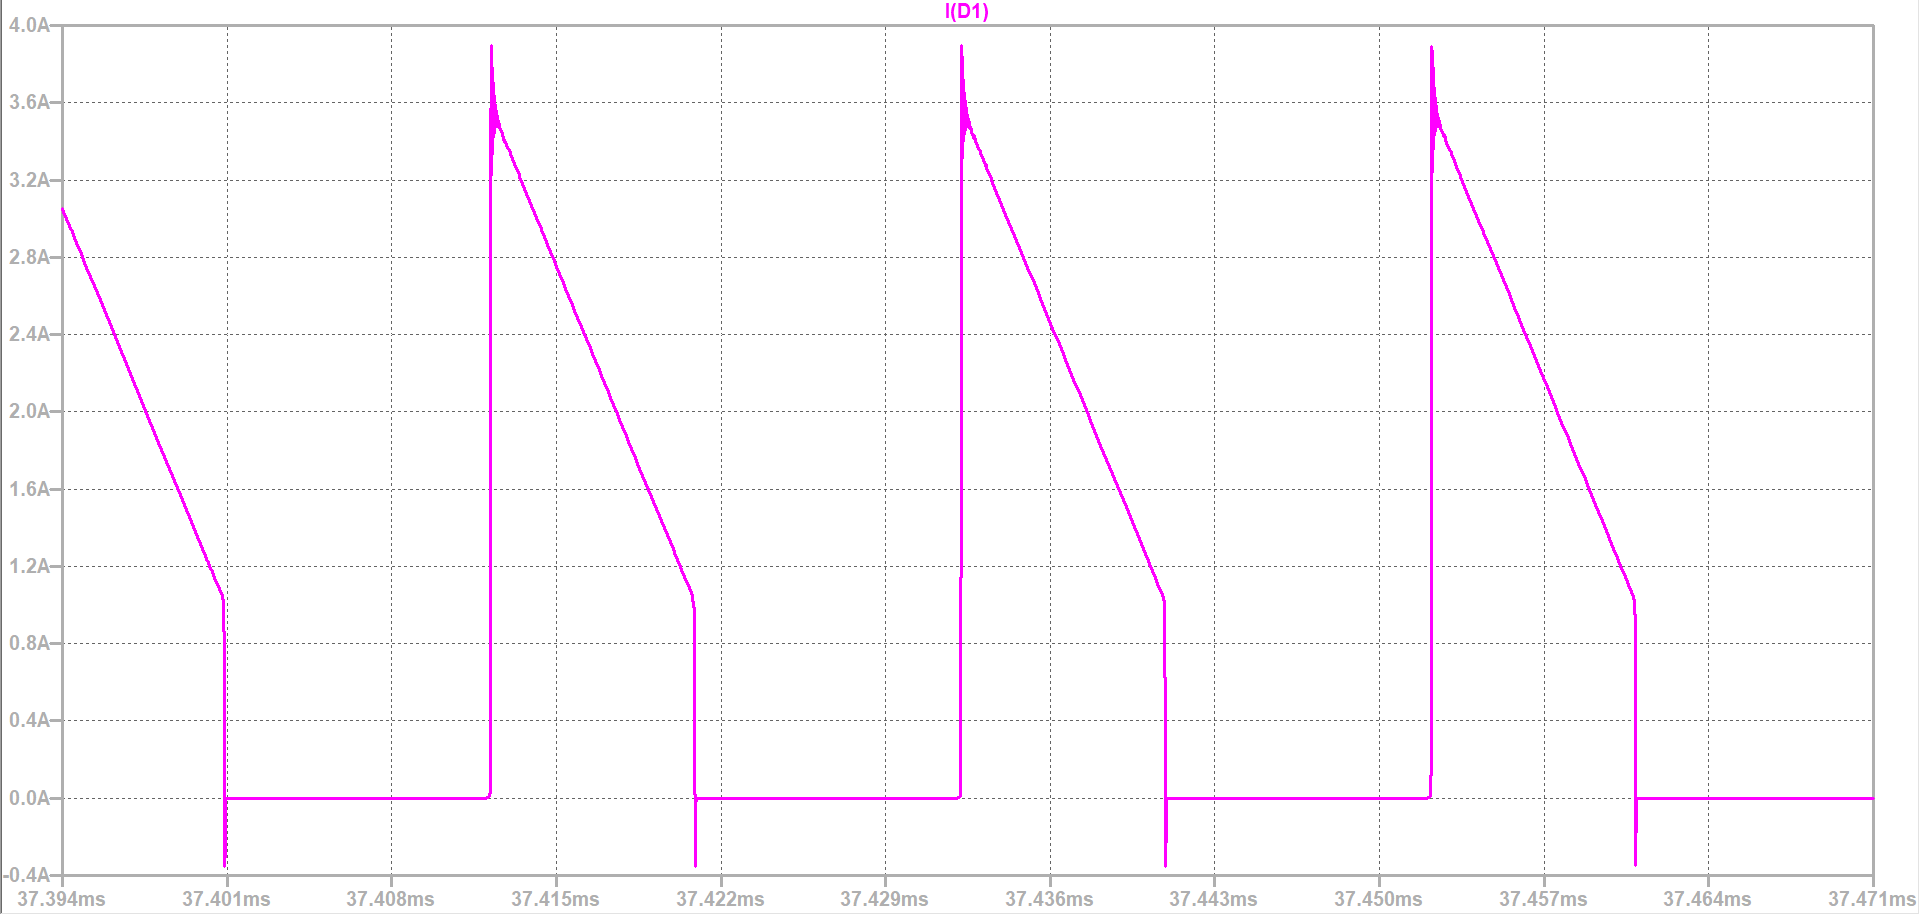
\includegraphics[width=0.6\textwidth]{Figures/diode-current.png}
    \caption{$I_{D_1}$ waveform with parasitic included.}
    \label{fig:i_d}
\end{figure}

\section{Component Selection}
Other components of the isolated SEPIC converter is selected as given below. Considering the requirements of the topology and safety measures, we have selected potential candidates for the components.

\subsection{Controller Selection}
For the duty cycle calculation against the variation in input and output sides, and therefore gathering the current and voltage measurements from the sensors, we have decided our controller to be a digital one and we have selected the STM32-Nucleo-F334R8 board. Related information about the controller is given in Table \ref{tab:controller}.

\begin{table}[H]
    \centering
    \caption{STM32-Nucleo-F334R8 board information.}
    \label{tab:controller}
    \begin{tabular}{|c|c|}
        \hline
        Supply voltage:         & 5 V / 7-12 V   \\
        \hline
        Max. CPU frequency:     & 72 MHz        \\
        \hline
        Dimensions in mm:       & 70x82.5       \\
        \hline
        Cost:                   & 330 TL        \\
        \hline
    \end{tabular}
\end{table}

\subsection{Sensors}
In order to adjust the duty cycle to compensate the changes in input and outputs of the converter, we should monitor the input and output voltages continuously. For this purpose we have selected an isolated Delta-Sigma modulator product for our voltage measurements. Its specifications are given in below Table \ref{tab:AMC}. This product gives separates input from the output via capacitive double isolation barrier. The device can also be used for current measurements. Additional shunt resistances are not mentioned in this section.

\begin{table}[H]
    \centering
    \caption{Isolated Delta-Sigma Modulator Specifications.\cite{web:AMC}}
    \label{tab:AMC}
    \begin{tabular}{|c|c|}
        \hline
        Part no:                & AMC1306M25DWVR    \\
        \hline
        Sampling rate:          & 78k/s             \\
        \hline
        Isolation strength:     & 7000 V            \\
        \hline
        Cost:                   & 143.5 TL          \\
        \hline
    \end{tabular}
\end{table}


\subsection{Switching Components}
Looking at the topology as given in Figure \ref{fig:iso_sepic}, we have two switching components which are the MOSFET at the primary side and the diode at the secondary side of the transformer. Looking at the simulation results in Section \ref{comp_simulation}, we have selected our switching components with the addition of safety factors. For the MOSFETs, we decided to parallel two MOSFET to decrease to losses due to $R_{ds,on}$.

\begin{table}[H]
    \centering
    \caption{MOSFET Specifications.\cite{web:mosfet}, will be paralleled.}
    \label{tab:mosfet}
    \begin{tabular}{|c|c|}
        \hline
        Part no:            &  RSS070N05FRA     \\
        \hline
        $V_{ds}$            &  45 V             \\
        \hline
        $I_d$               &  7 A              \\
        \hline
        $R_{ds,on}$         & 25 $m\Omega$      \\
        \hline
        Total gate charge:  & 12 nC             \\
        \hline
        Cost:               & 15.2 TL           \\
        \hline
    \end{tabular} 
\end{table}

To drive these MOSFETS properly, we have selected an isolated gate driver with specifications below in Table \ref{tab:gate_driver}.

\begin{table}[H]
    \centering
    \caption{Gate Driver Product Specifications.\cite{web:gate_driver}}
    \label{tab:gate_driver}
    \begin{tabular}{|c|c|}
         \hline
         Part no:               & UCC23313BDWYR     \\
         \hline
         Current output peak:   & 5.3 A             \\
         \hline
         Output supply:         & 14-33 V           \\
         \hline
         Cost:                  & 33.1 TL           \\
         \hline
    \end{tabular}
\end{table}

For the diode, we have selected the following Schottky diode product for our design as given below. Again we are not limited to this product, we can select another Schottky diode with similar ratings for our design if this one is not available during the implementation.

\begin{table}[H]
    \centering
    \caption{Schottky Diode Specifications.\cite{web:diode}}
    \label{tab:diode}
    \begin{tabular}{|c|c|}
        \hline
        Part no:            & VSSAF512          \\
        \hline
        $V_r$               & 12 V              \\
        \hline
        $I_f$               & 5 A               \\
        \hline
        $V_{f,max}$         & 0.88 V            \\
        \hline
        Cost:               & 7.6 TL            \\
        \hline
    \end{tabular}
\end{table}


\subsection{Inductor Core Selection}
For the inductor at the input side, in order not to saturate the core and obtain the desired inductance value, we have selected a Kool Mu core with its specifications below. Again we will be looking for alternative cores for our inductor design, considering our available space and limitations.

\begin{table}[H]
    \centering
    \caption{Inductor Toroid core specifications.\cite{web:tor_core}}
    \label{tab:toroid_core}
    \begin{tabular}{|c|c|}
        \hline
        Part no:            & 0077548A7         \\
        \hline
        Core material:      & Kool Mu           \\
        \hline
        Permeability:       & 125               \\
        \hline
        Inductance Ratio:   & 127 $nH/T^2$      \\
        \hline
        Dimensions in mm:   & 33x33x11          \\
        \hline
        Cost:               & 52 TL             \\
        \hline
    \end{tabular}
\end{table}

If we select and wind this core with $N=16$ turns to get a $32.6\mu H$ inductor with AWG26 wire with the same paralleling configuration for the primary side, we get the ESR of the inductance as given below. Using the core dimensions, an estimate length for each winding is calculated as 48 mm.

\begin{equation}
    ESR_{L}=\frac{48 mm\times16\times133 m\Omega/m\times10^{-3}m/mm}{12}=8.6 m\Omega
\end{equation}

\subsection{Capacitor Selection}
Selecting the input capacitor, we desired a large enough capacitor with enough current rating. We have decided on paralleling three of the Aluminum capacitor with given parameters in Table \ref{tab:input_cap}. Since we are paralleling the capacitors, if the component will not be available, we can select smaller capacitance with similar ratings but this will result in higher volumes of the converter.

\begin{table}[H]
    \centering
    \caption{Input Capacitor Specification.\cite{web:input_cap}}
    \label{tab:input_cap}
    \begin{tabular}{|c|c|}
        \hline
        Part no:        & KR3-035V332MJ250  \\
        \hline
        Capacitance:    & 3300 $\mu F$      \\
        \hline
        Rated voltage:  & 35 $V$             \\
        \hline
        Ripple current: & 1960 $mA$         \\
        \hline
        Dimensions in mm & 16x16x25          \\
        \hline
        ESR:            & not specified     \\
        \hline
        Cost:           & 11 TL             \\
        \hline
    \end{tabular}
\end{table}

For the output capacitor, since the output voltage ripple is desired to be very low, we agreed on putting a 1 mF capacitor to the output side. Parameters of the candidate capacitor is given below. We are not limited to using this capacitor, we can select another one with similar ratings in case of unavailability.

\begin{table}[H]
    \centering
    \caption{Output Capacitor Specification.\cite{web:output_cap}}
    \label{tab:output_Cap}
    \begin{tabular}{|c|c|}
        \hline
        Part no:        & KLH-100V102MK400  \\
        \hline
        Capacitance:    & 1000 $\mu F$      \\
        \hline
        Rated Voltage:  & 100 V             \\
        \hline
        Ripple current: & 2500 $mA$         \\
        \hline
        ESR:            & 76 $m\Omega$      \\
        \hline
        Dimensions(mm)  & 18x18x40          \\
        \hline
        Cost:           & 23.3 TL           \\
        \hline
    \end{tabular}
\end{table}

\section{Loss Analysis}
In this section the losses of the isolated SEPIC converter design, are calculated. For the calculations, steady state operation and below operation conditions are utilized. Losses on the MOSFET, diode, transformer and the input inductor are calculated. Summing up the below calculations, we have a total loss of  4.74 W. Also note that switching losses (gate opening and closing) are ignored compared to other losses.

\begin{table}[H]
    \centering
    \caption{Operating Conditions for Loss Calculation.}
    \label{tab:los_conditions}
    \begin{tabular}{|c|c|}
        \hline
        Switching Frequency:        & 50 kHz    \\
        \hline
        Duty Cycle:                 & 0.5       \\
        \hline
        Input Voltage:              & 16 V      \\
        \hline
    \end{tabular}
\end{table}

\subsection{MOSFET Conduction Losses}
\begin{equation}
    P_{MOS} = I^2R_{ds,on}D = 8^2\times25\times10^{-3}\times0.5 = 0.8 W
\end{equation}

\subsection{Diode Conduction Losses}
\begin{equation}
    P_{diode} = I_oV_f(1-D) = 2.25\times0.88\times0.5 = 1 W
\end{equation}

\subsection{Transformer Core and Conduction Losses}
Since we are working in CCM with a switching frequency $f_{sw}=50 kHz$, we have a core loss at most the quarter of the loss indicated in the datasheet \cite{web:ferrite_cores}.

\begin{equation}
    P_{core,tr} = \frac{1}{4}\times6 = 1.5 W
\end{equation}

For the conduction losses on the transformer, the average currents for (1-D) period is calculated from the simulation results.

\begin{equation}
    I_{s,avg} = 2.25 A
\end{equation}
\begin{equation}
    I_{p,avg} = 2.25\times3.2 = 7.2 A
\end{equation}
\begin{equation}
    P_{cond,tr} = P_{primary} + P_{secondary} = (I^2_{p,avg}\times R_p + I^2_{s,avg}\times R_s)(1-D)
\end{equation}
\begin{equation}
    P_{cond,tr} = 0.3 W
\end{equation}

\subsection{Inductor Core and Conduction Losses}
Looking at the toroid core datasheet, we have a $750mW/cm^3$ for 100 kHz and the core volume is 5.34 $cm^3$, giving 4 W for this core. Again we can assume quarter of this loss as a core loss since we work with 50 kHz and CCM.
\begin{equation}
    P_{core,ind} = 1 W
\end{equation}
\begin{equation}
    P_{cond,ind} = I^2_{in,avg}ESR_{ind} = 0.14 W
\end{equation}

\subsection{Efficiency Calculation for Different Load Cases}
Above calculations are done for the 100\% loading case where the output current is 1 A. For the 75\%,50\% and 25\% loading cases, we can calculate the losses easily since the all the current averages will be the respective percentages of the loading cases. Therefore conduction ($I^2R$) losses will change by the square of the loading whereas the core losses will change by the loading percentage. Diode losses also will change by the loading percentage. Resulting efficiency table shows the results.

\begin{table}[H]
    \centering
    \caption{Efficiency results of different cases.}
    \label{tab:eff}
    \begin{tabular}{|c|c|c|c|}
        \hline
        Loading percentage  & $P_{loss}$    & $P_{out}$ & Efficiency    \\
        \hline\hline
        100\%               & 4.74 W        & 48 W      & 91.01\%       \\
        \hline
        75\%                & 3.32 W        & 36 W      & 91.55\%       \\
        \hline
        50\%                & 2.06 W        & 24 W      & 92.1\%        \\
        \hline
        25\%                & 0.95 W        & 12 W      & 92.66\%       \\
        \hline
    \end{tabular}
\end{table}

\newpage
\section{Conclusion}
In this report, design selections and selected components for the selected topology, are given. Magnetic design calculations and overall simulation results with both ideal and non-ideal components are given. Looking at the simulation results we observed some facts about our design. There are significant differences between the ideal and non-ideal simulation results. For instance, idealized duty calculation does not give the required duty for desired output voltage due to losses and drops on the non-idealities of the components. Also considering the starting operation, there might be overshoots on the components that could damage them. We will be more cautious about the non-idealities and further investigate alternative components to reduce the non-ideality effects on the topology. 

\newpage
\bibliographystyle{IEEEtran}
\bibliography{ref.bib}

\end{document}